\section{Mechanistic Probes: What Does EGPT Learn?}
\label{sec:probes}
%% ============================================================

\subsection{Helmholtz Decomposition of Projection Matrices}

Any square matrix $W \in \mathbb{R}^{d \times d}$ decomposes as $W = S + A$, where
$S = (W + W^\top)/2$ (symmetric, gradient component) and $A = (W - W^\top)/2$
(anti-symmetric, curl component).
For an energy function, a pure gradient projection requires $W = S$ ($\rho = 0$),
while a pure rotation requires $W = A$ ($\rho \to \infty$).
A random matrix has $\rho = \|A\|_F / \|S\|_F = 1$ by symmetry.

\begin{figure}[h]
  \centering
  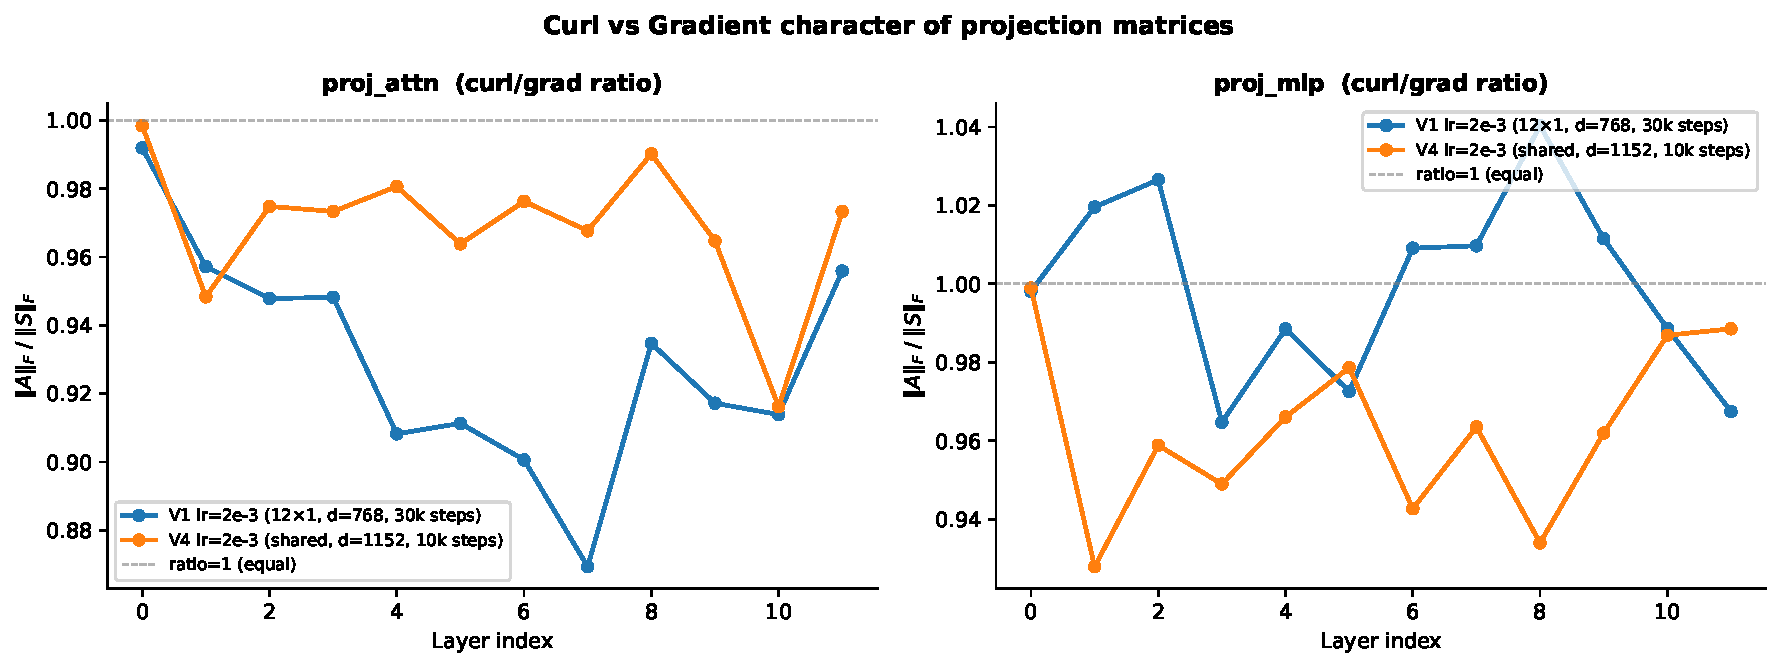
\includegraphics[width=0.92\textwidth]{../results/multi-block-ablation/plots/curl_grad_ratio.pdf}
  \caption{Per-layer curl-to-gradient ratio for the attention and MLP projection matrices.
    V1 EGPT (trained, $d=768$): $\rho_{\mathrm{attn}}=0.930$, $\rho_{\mathrm{mlp}}=1.000$.
    V4 EGPT (trained, $d=1152$): $\rho \in [0.93, 0.99]$ throughout.
    Both models converge to balanced Helmholtz decomposition ($\rho \approx 1$),
    regardless of initialisation or model size.}
  \label{fig:curl_grad}
\end{figure}

\paragraph{Finding.}
Trained EGPT models spontaneously learn balanced projections ($\|S\|_F \approx \|A\|_F$).
A mild gradient bias in the attention stream ($\rho < 1$) is consistent with the
inductive bias toward dissipation in iterative inference.
The balance is \emph{emergent}: starting from random initialisation ($\rho = 1$),
training maintains the balance over 30k steps.
Explicitly forcing the balance (V6--V8) is significantly worse, suggesting the
projection policy needs unconstrained freedom to decide how much curl vs.\ gradient
to apply at each layer.

\subsection{Layer Similarity: Is There a Shared Energy Function?}

A central claim of EGPT is that all blocks perform gradient steps on a \emph{shared}
energy function.  If true, the pre-projection attention outputs
$\mathrm{attn\_out}^{(i)} = \mathrm{attn}(\mathrm{LN}(h^{(i)}))$ (the gradient signal
before the policy is applied) should be more similar across layers than in GPT.

We compare three models on a 512-token WikiText prefill, measuring Linear CKA and
cosine similarity of per-component inter-layer similarities.

\begin{table}[h]
\centering
\caption{Mean off-diagonal inter-layer similarity for four components.
  ``Random'' = untrained V1 EGPT.  CKA is dominated by the shared residual stream
  and is a poor probe; cosine similarity is correctly near-zero for the random baseline.}
\label{tab:layer_sim}
\small
\begin{tabular}{llccc}
\toprule
\textbf{Component} & \textbf{Metric} & \textbf{V1 EGPT} & \textbf{V0 GPT} & \textbf{Random} \\
\midrule
h\_out (residual)     & CKA    & 0.663 & 0.572 & 0.952 \\
                      & Cosine & \textbf{0.764} & 0.612 & 0.670 \\
attn\_out (grad$_E$)  & CKA    & 0.463 & 0.326 & 0.961 \\
                      & Cosine & \textbf{0.176} & 0.119 & 0.006 \\
ffwd\_out (grad$_E$)  & CKA    & 0.513 & 0.367 & 0.891 \\
                      & Cosine & $-0.000$ & 0.078 & $-0.002$ \\
update ($\Delta x$)   & CKA    & 0.380 & \textbf{0.383} & 0.849 \\
                      & Cosine & 0.022 & \textbf{0.085} & $-0.001$ \\
\bottomrule
\end{tabular}
\end{table}

\begin{figure}[h]
  \centering
  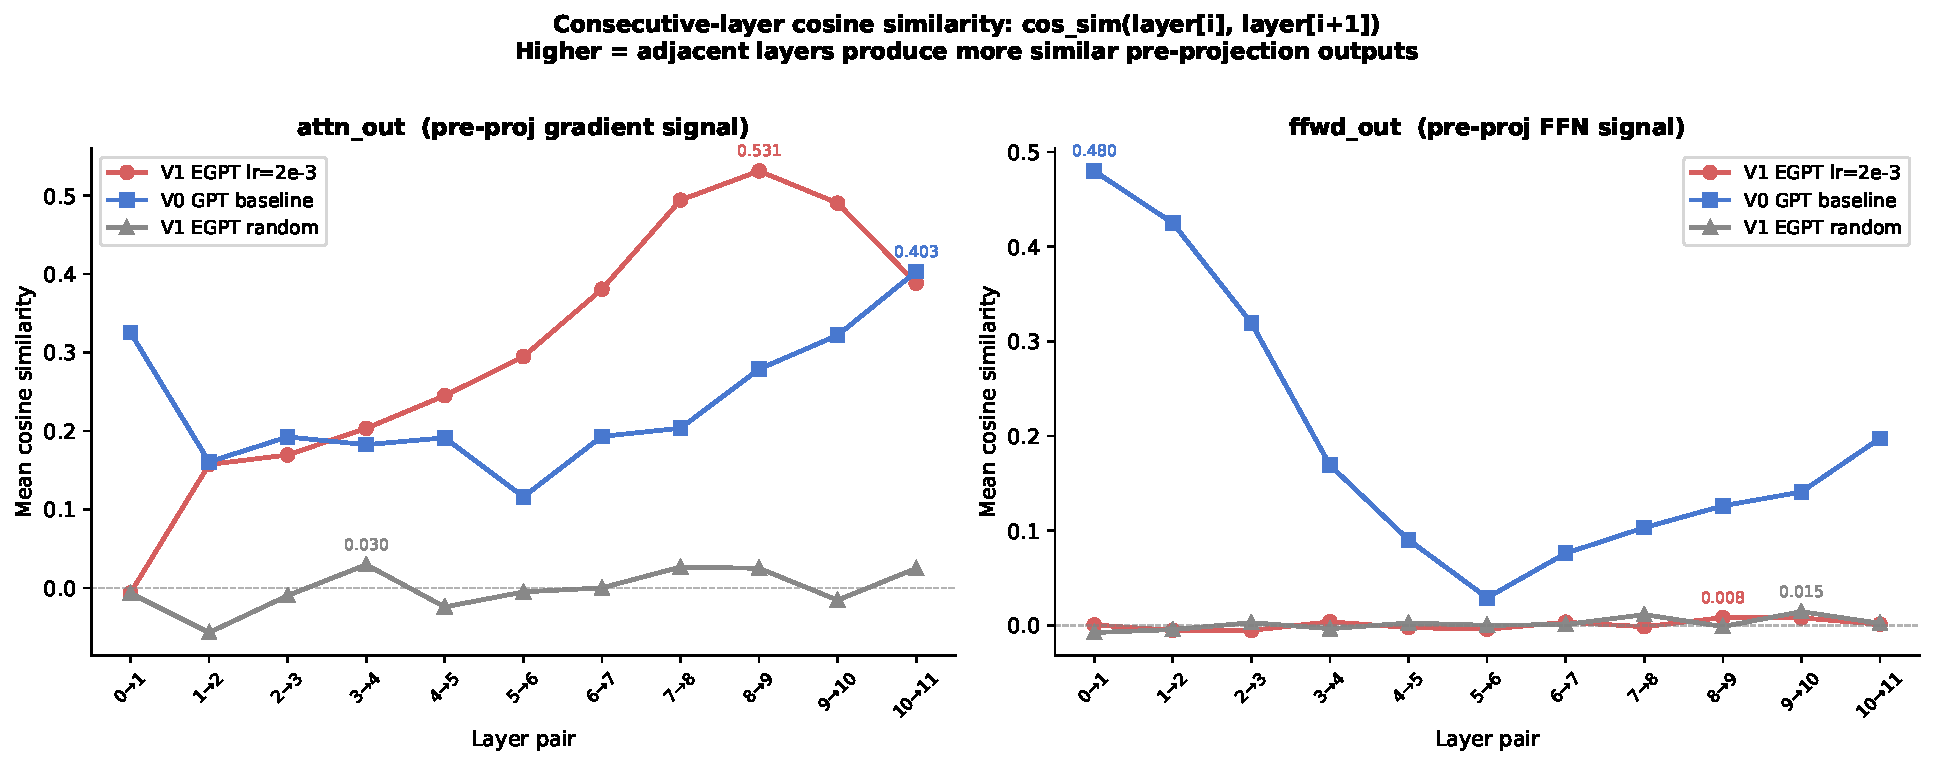
\includegraphics[width=\textwidth]{../results/multi-block-ablation/plots/consecutive_layer_sim.pdf}
  \caption{Consecutive-layer cosine similarity for attention (left) and FFN (right) pre-projection outputs.
    V1 EGPT attention similarity rises monotonically to 0.531 at layers 8--9 (far above GPT's $\le$0.40),
    then plateaus.  FFN similarity is near zero for EGPT throughout.}
  \label{fig:consecutive_layer_sim}
\end{figure}

\paragraph{Key findings.}
\begin{itemize}
  \item \textbf{Attention gradient is shared, FFN gradient is not.}
    V1 EGPT shows attention cosine 0.176 vs.\ GPT 0.119 and random 0.006.
    FFN cosine is $-0.000$ for EGPT (comparable to random $-0.002$),
    while GPT has 0.078.
    The shared-energy interpretation holds only for the attention stream.

  \item \textbf{Monotonic rise to convergence in later layers.}
    Consecutive-layer attention cosine in V1 EGPT rises from $\approx 0$ at layers 1--2
    to a peak of 0.531 at layers 8--9, then slightly declines.
    Layers 6--10 are strong candidates for weight-sharing based on this metric.

  \item \textbf{CKA is dominated by input geometry.}
    The untrained random model has the \emph{highest} CKA (0.85--0.96) because all layers
    receive the same embedded input.  Training reduces CKA by specialising layers.
    CKA should not be used to test the shared-energy hypothesis in this setting.

  \item \textbf{Residual stream converges: EGPT $>$ GPT.}
    EGPT's residual-stream cosine (0.764) exceeds GPT's (0.612) and the random baseline (0.670),
    consistent with convergent gradient dynamics pulling $h$ toward a common attractor.
\end{itemize}

\subsection{Layer Merging: Why High Similarity Does Not Imply Mergeability}

Given the high consecutive-layer cosine similarity in EGPT (layers 8--9: 0.531),
one might hope to merge adjacent blocks via weight averaging without performance loss.

\begin{figure}[h]
  \centering
  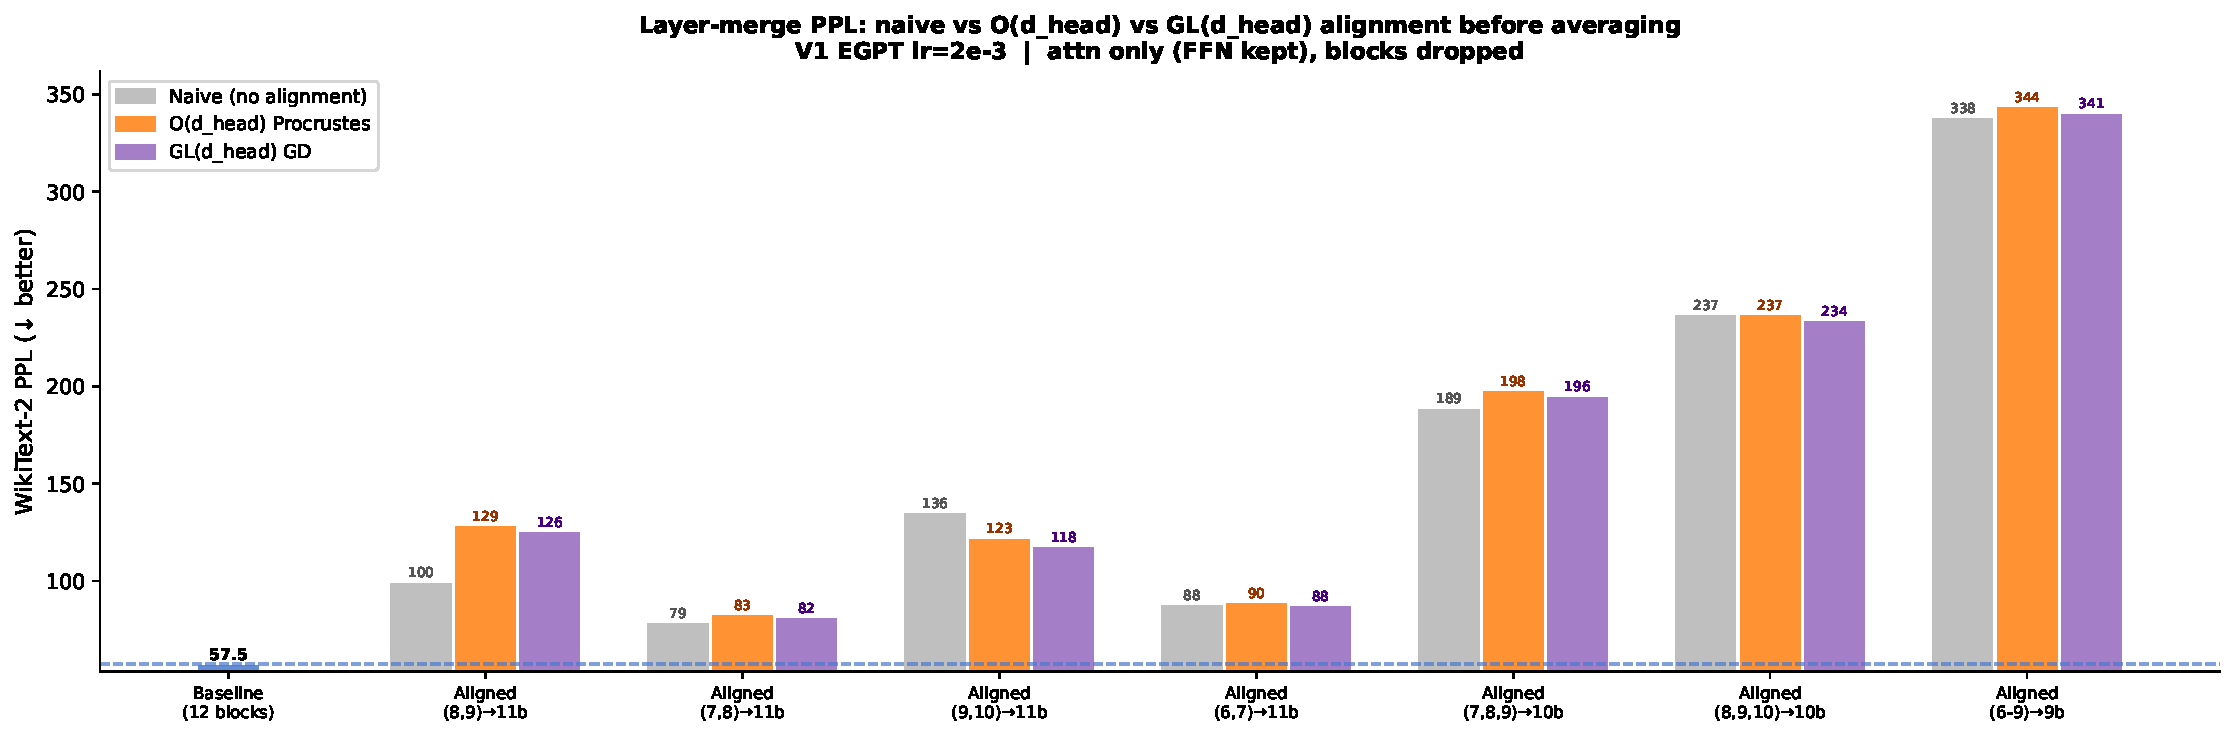
\includegraphics[width=\textwidth]{../results/multi-block-ablation/plots/layer_merge_aligned_ppl.pdf}
  \caption{WikiText PPL for layer merges: naive (grey), O($d_h$) Procrustes (orange),
    and GL($d_h$) gradient descent (purple).
    Neither alignment strategy consistently recovers the loss.  The best single-pair merge
    (7--8: +38\% PPL) is far from lossless.}
  \label{fig:layer_merge_aligned_ppl}
\end{figure}

\paragraph{Result.}
Even the best single-pair merge (layers 7--8, second-highest cosine similarity) increases
PPL by 38\% (57.51 $\to$ 79.25).
The pair with highest cosine (8--9) shows the worst merge (+74\%).
GL($d_h$) alignment (full scaling and shear, not just rotations) provides at most 4\%
improvement over naive averaging.

\paragraph{Interpretation.}
The high output-space cosine similarity is a property of the \emph{function} computed,
not of the \emph{weights}.
EGPT's subtractive update keeps $h$ near a shared attractor, so each layer sees similar
inputs and computes similar directions --- but the weight matrices themselves are not
structurally related.
High functional similarity does not imply structural redundancy:
zero-shot weight merging is not a viable compression strategy for EGPT.
Fine-tuning after merge, or block-drop (keeping one block intact), remain viable alternatives.

\subsection{EGrad and EDesc: Layer Similarity at Both Scales}
\label{sec:layer_sim_egrad}

MixH (V15, V16, V19, V20; intended as EGrad/EDesc but trained as MixedHead) use a fundamentally different block structure:
mixed heads with a shared output projection and an additive (EGrad) or subtractive (EDesc)
residual update.
We extend the layer similarity analysis to these models.

\begin{table}[h]
\centering
\caption{Off-diagonal mean cosine similarity at d=768 (12$\times$1) and d=1024 (24$\times$1).
  Highest per row in each group \textbf{bold}.}
\label{tab:layer_sim_egrad}
\small
\setlength{\tabcolsep}{5pt}
\begin{tabular}{lc@{\quad}cccc@{\quad\quad}ccc}
\toprule
& & \multicolumn{4}{c}{\textbf{d=768 (small scale)}} & \multicolumn{3}{c}{\textbf{d=1024 (400M)}} \\
\cmidrule(lr){3-6} \cmidrule(lr){7-9}
\textbf{Component} & & V0 GPT & V1 EGPT & V15 Mixed & V16 Mixed & V9 GPT & V19 Mixed & V20 Mixed \\
\midrule
attn\_out  & & 0.121 & \textbf{0.216} & 0.107 & 0.106 & 0.093 & 0.094 & \textbf{0.095} \\
ffwd\_out  & & 0.080 & 0.000 & \textbf{0.157} & 0.158 & \textbf{0.267} & 0.116 & 0.126 \\
update ($\Delta x$) & & 0.088 & 0.026 & \textbf{0.168} & 0.163 & \textbf{0.235} & 0.106 & 0.119 \\
\bottomrule
\end{tabular}
\end{table}

\begin{figure}[ht]
  \centering
  \begin{subfigure}[b]{\textwidth}
    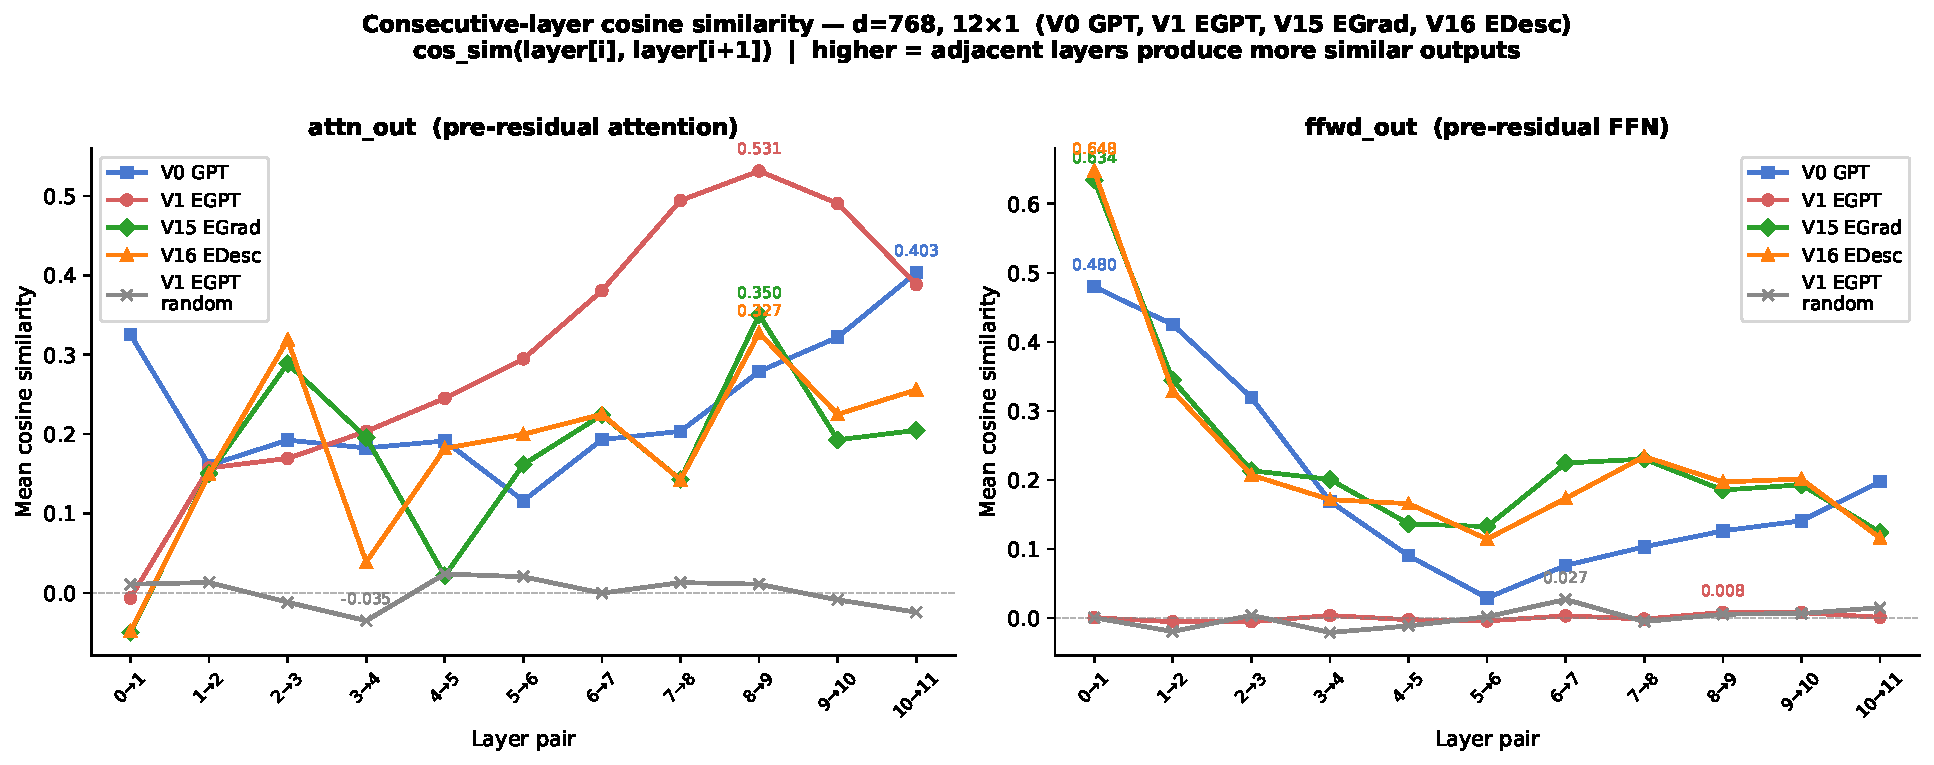
\includegraphics[width=\textwidth]{../results/multi-block-ablation/plots/consecutive_sim_small.pdf}
    \caption{d=768, 12 layers.  Left: attn\_out — V1 EGPT peaks at 0.531; MixH stay below
      GPT ($\le$0.350).  Right: ffwd\_out — MixH show high early-layer FFN similarity
      (consecutive max 0.634/0.648), while V1 EGPT is near zero.}
    \label{fig:consecutive_small}
  \end{subfigure}
  \vspace{4pt}
  \begin{subfigure}[b]{\textwidth}
    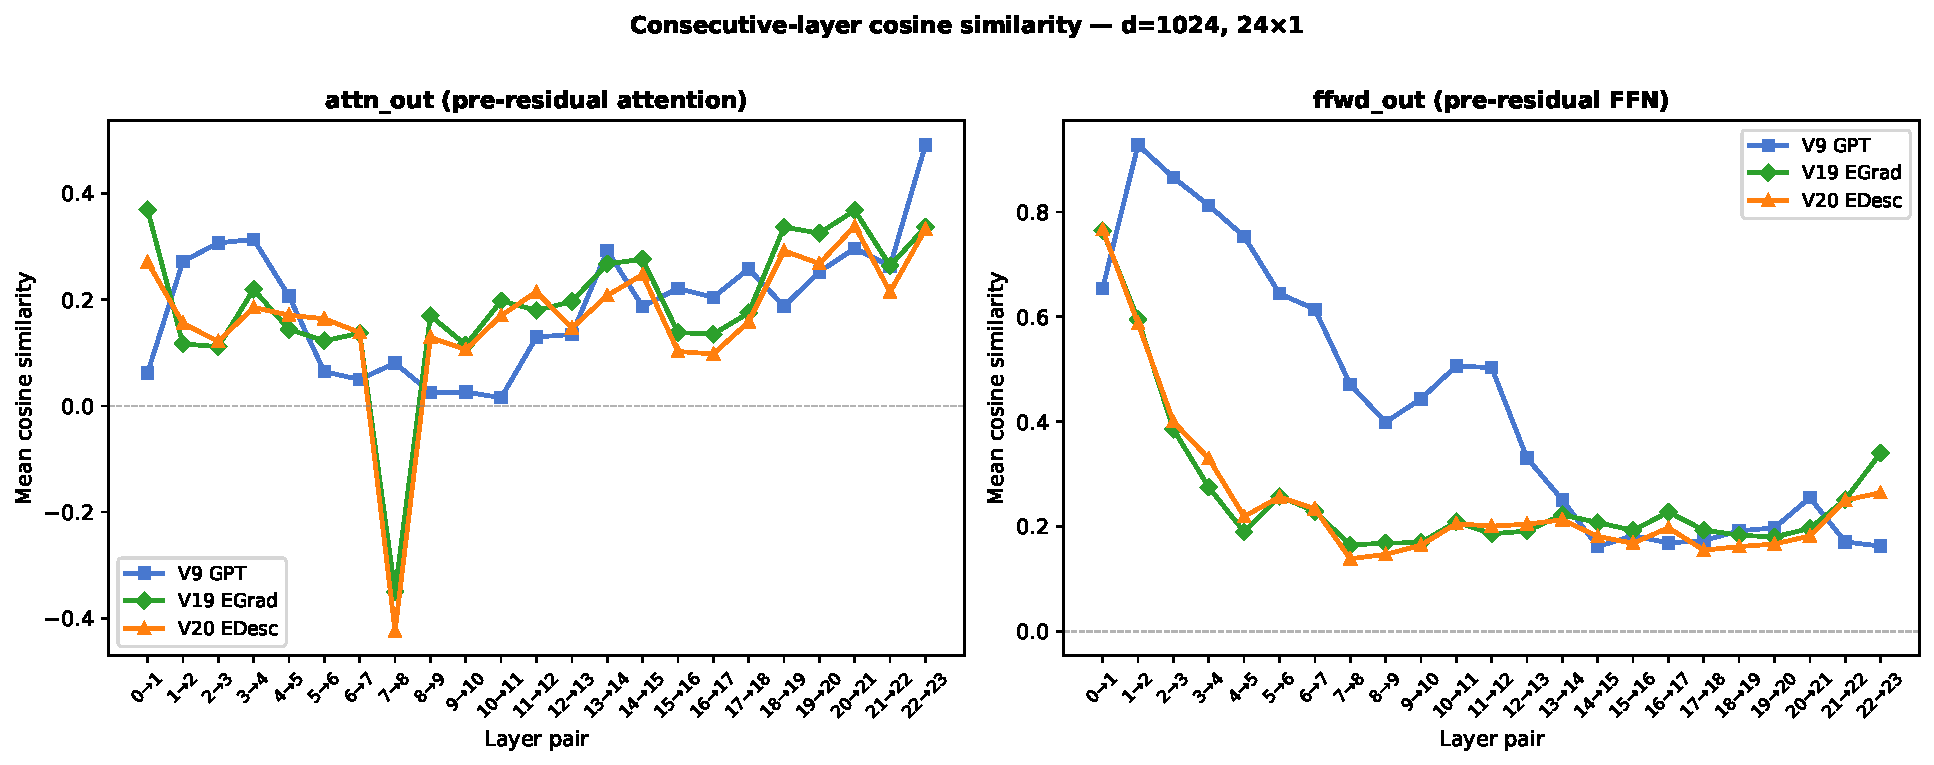
\includegraphics[width=\textwidth]{../results/multi-block-ablation/plots/consecutive_sim_400m.pdf}
    \caption{d=1024, 24 layers.  Attn\_out: all three models near-identical.
      FFN: V9 GPT starts at 0.928 (pair 0--1) and decays; MixH remain well below.}
    \label{fig:consecutive_400m}
  \end{subfigure}
  \caption{Consecutive-layer cosine similarity at both scales.}
  \label{fig:consecutive_both}
\end{figure}

\begin{figure}[ht]
  \centering
  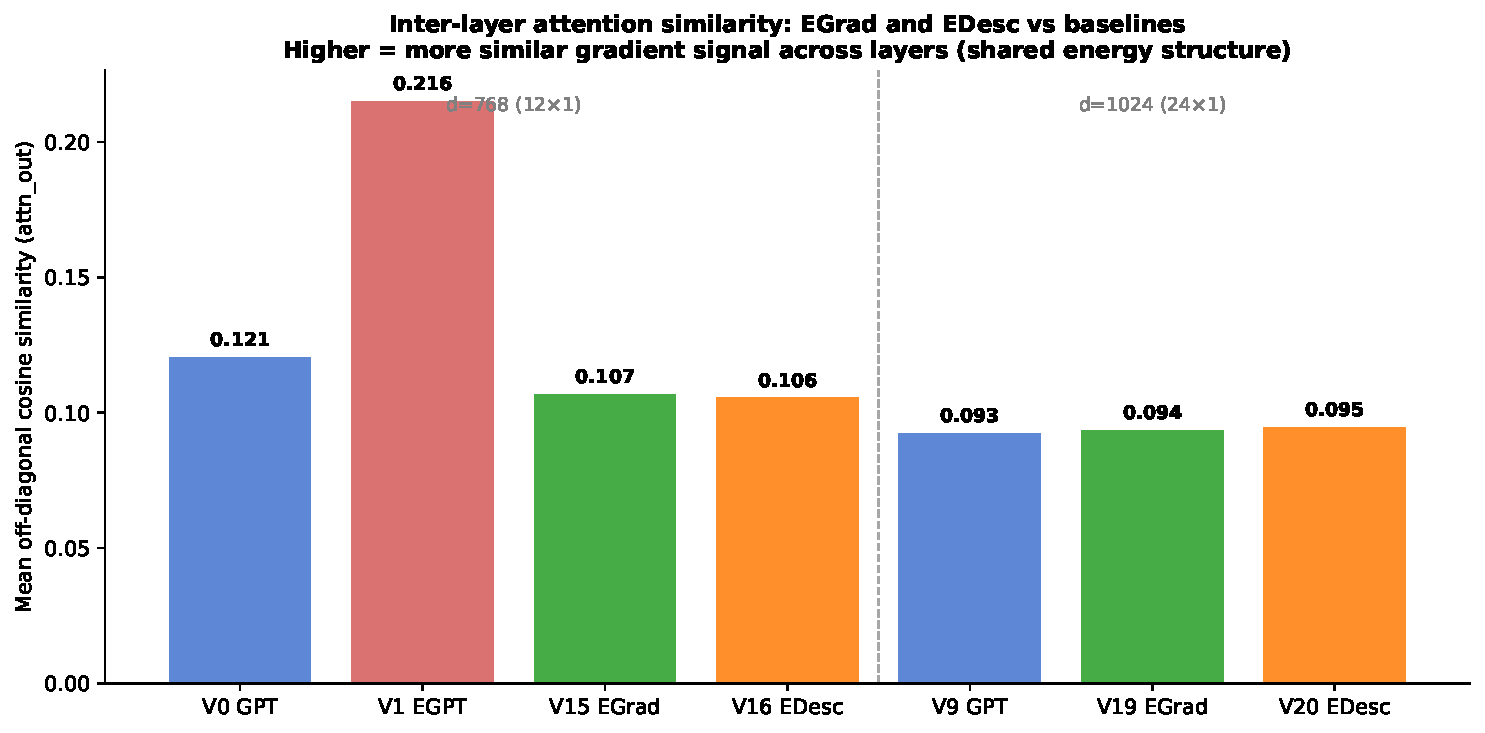
\includegraphics[width=0.7\textwidth]{../results/multi-block-ablation/plots/layer_sim_summary_egrad_edesc.pdf}
  \caption{Off-diagonal mean attn\_out cosine similarity across all models.
    V1 EGPT (0.216) leads; MixH (V15/V16) ($\approx$0.107) are below GPT (0.121).
    At 400M scale (right group), all three architectures converge to $\approx$0.094.}
  \label{fig:layer_sim_summary_egrad}
\end{figure}

\begin{figure}[ht]
  \centering
  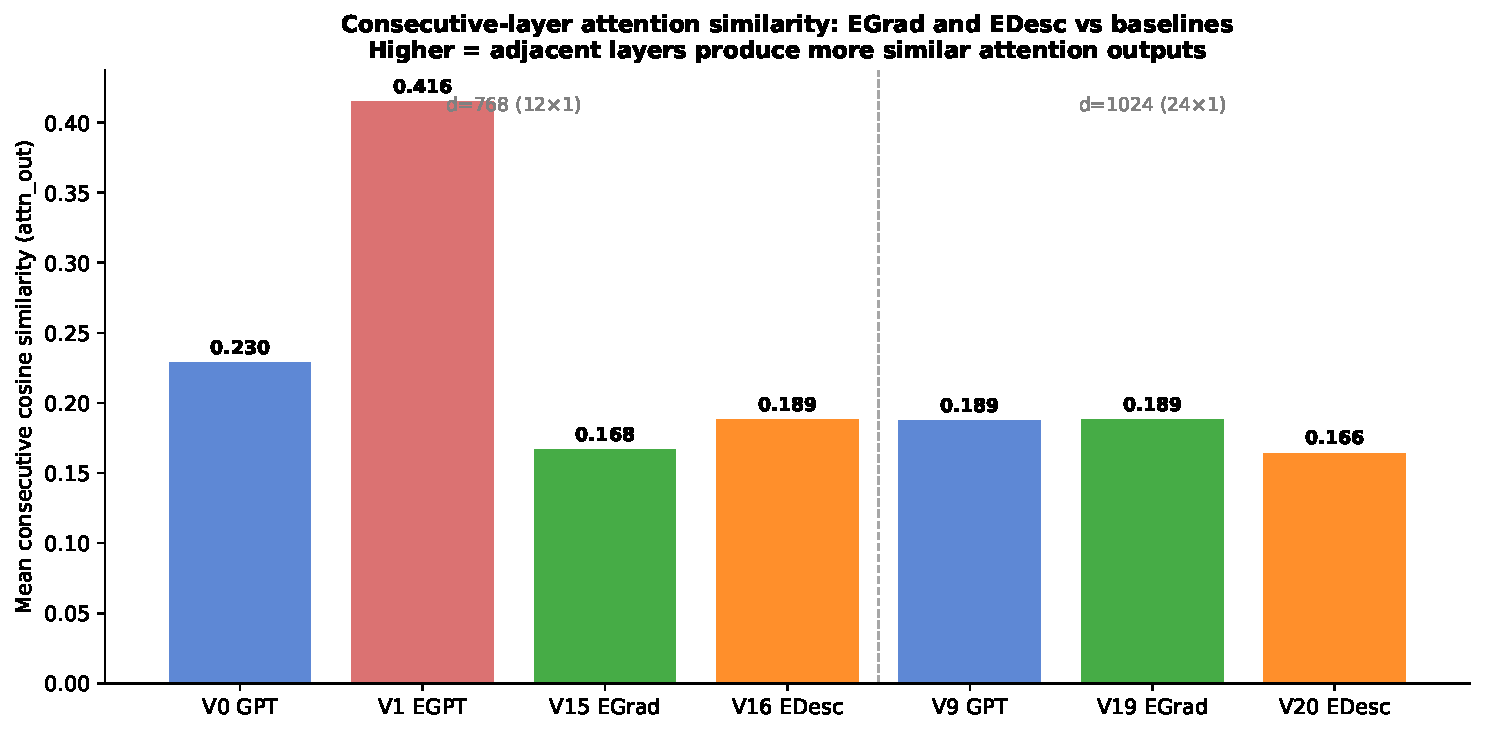
\includegraphics[width=0.7\textwidth]{../results/multi-block-ablation/plots/layer_sim_summary_egrad_edesc_consec.pdf}
  \caption{Consecutive-layer mean attn\_out cosine similarity (adjacent pairs only).
    Same trend as the off-diagonal mean: V1 EGPT has highest consecutive alignment.}
  \label{fig:layer_sim_summary_egrad_consec}
\end{figure}

\paragraph{Three findings.}
\begin{enumerate}
  \item \textbf{MixH do not inherit V1 EGPT's shared-attention structure.}
    V1 EGPT's high attn cosine (0.216) arises from the $V{=}K$ constraint causing
    attention outputs to converge to a shared key-space direction in later layers.
    MixH mix these heads with standard GPT heads, breaking the convergence:
    attn off-diagonal drops to 0.107/0.106, \emph{below} V0 GPT (0.121).

  \item \textbf{FFN similarity inverts.}
    V1 EGPT's aggressive subtractive update causes the residual stream to vary sharply
    between layers, producing near-zero FFN cross-layer cosine ($\approx$0).
    MixH.s gentler updates keep $h$ in a more stable regime: FFNs see similar
    inputs at adjacent layers, producing ffwd cosine of 0.157/0.158 and consecutive
    peaks of 0.634--0.648.  The pattern flips entirely: where V1 EGPT has shared
    attention, MixH have shared FFN.

  \item \textbf{Update coherence peaks for EGrad/EDesc.}
    The step $\Delta x$ is most cross-layer consistent for MixH-A (0.168) and
    MixH-B (0.163), far above V1 EGPT (0.026) and GPT (0.088).
    EGrad/EDesc apply a globally coherent update direction across all layers.

  \item \textbf{At 400M scale, GPT's FFN becomes highly redundant.}
    V9 GPT shows consecutive FFN cosine of 0.928 at layer pair 0--1, decaying to
    $\sim$0.4 across depth --- suggesting early FFN layers in the 400M GPT are nearly
    identical.  MixH.s FFN diversity (0.116/0.126 off-diag) may be one reason
    they outperform GPT: more diverse FFN representations across depth.
\end{enumerate}

%% ============================================================
